% Este arquivo .tex será incluído no arquivo .tex principal. Não é preciso
% declarar nenhum cabeçalho

\section{CACo -- Centro Acadêmico da Computação}

\begin{figure}[H]
  \centering
  \includegraphics[width=.35\textwidth]{img/caco_logo.pdf}
\end{figure}

\subsection{O que é um centro acadêmico?}

Bixete, o CACo é o seu centro acadêmico. Um CA é uma entidade estudantil que,
em linhas gerais, deve trabalhar para garantir os interesses de todas e todos
estudantes, melhorando o curso e a faculdade a que pertence. Qualquer pessoa
que se encaixa na descrição anterior é um membro do CACo e isso inclui você.
O CACo é formado pelas alunas e alunos de graduação tanto em engenharia quanto
em ciência da computação da Unicamp, além de pessoas da pós-graduação do IC.

Um centro acadêmico é parte do famoso ``movimento estudantil'' de que você
provavelmente já ouviu falar. Mas não se engane! Pergunte para o seu pai o que
ele pensa quando lê ``movimento estudantil'' e ele vai dizer que vê um bando de
estudantes desocupadas e desocupados associadas a um partido político de
esquerda que saem por aí protestando contra o sistema e queimando ônibus pelas
ruas. Se você pensa assim, mude sua ideia: o CACo não é nada disso.

\begin{figure}[H]
  \centering
  \includegraphics[width=.45\textwidth]{img/alem_da_graduacao/caco_karaoke.jpg}
\end{figure}

O CACo tem como função representar estudantes no âmbito acadêmico, ou seja,
perante o IC, a FEEC e a Unicamp. Mas o que o CACo faz? De forma simplificada,
procuramos ser porta-voz de alunas e alunos. Reivindicamos espaço físico
decente, alteração nas matérias e seus oferecimentos, promovemos discussões
sobre temas polêmicos e delicados, mas também integração e muitas outras
atividades.

Quer um exemplo? Esse estupendo manual que você está lendo neste exato momento
foi confeccionado pelo seu centro acadêmico para lhe ajudar no início da sua
vida universitária e, na verdade, você ainda vai se pegar recorrendo ao seu
manual várias vezes durante seus quatro, cinco, doze anos na Unicamp.

Uma grande função do CACo é prezar pela qualidade dos cursos e fazemos isso,
por exemplo, através de discussões com o próprio Instituto, onde levamos
reclamações e reivindicações para as coordenadoras, professoras, os
coordenadores e professores.

\begin{figure}[H]
  \centering
  \includegraphics[width=.45\textwidth]{img/alem_da_graduacao/caco_reuniao.jpg}
\end{figure}

Uma outra função do CACo é integrar estudantes de computação da Unicamp. Para
isso, realizamos diversos eventos como o CineCACo, o PipoCACo, o CACo Games,
o MagiCACo e a grande comemoração do Aniversário do CACo, que já contou com
pizza de graça para mais de duzentas pessoas! Tentamos também facilitar a vida
da galera através dos armários que alugamos, o banco de livros e o maravilhoso
banco de provas, provavelmente o maior da Unicamp, disponível online.

Repetindo o que foi dito antes: bixete, o CACo é o \textbf{SEU} centro
acadêmico. Tudo que dissemos que fazemos pelas alunas e alunos, queremos fazer
por você também. Por isso, quando houver algum problema envolvendo a FEEC, o
IC, as professoras, os professores ou qualquer coisa do tipo, não hesite em nos
procurar. O CACo sempre lhe dará todo o suporte necessário. Se tiver reclamação
ou sugestão relacionada ao próprio CACo, também estaremos aqui para ouvir. Mais
do que isso, venha participar de uma de nossas reuniões, que são abertas a você
e todas as alunas e alunos de computação da Unicamp.

\begin{figure}[H]
  \centering
  \includegraphics[width=.45\textwidth]{img/alem_da_graduacao/caco_fisl2.jpg}
\end{figure}

\subsection{Como posso participar do centro acadêmico?}

Participar do CACo é uma experiência diferente de tudo aquilo que você terá na
sua graduação. É a chance de aprender e crescer de uma forma que não acontece
em nenhuma aula de cálculo. É uma oportunidade de conhecer suas veteranas e
veteranos, além de suas colegas bixetes e seus colegas bixos. Mas, acima de
tudo, é uma experiência pessoal onde você vai aprender a se expressar,
argumentar, defender suas ideias, falar em público e pensar no coletivo. Você
entrará em contato com muita gente que provavelmente você nunca iria conhecer
e, com certeza, fará amizade com muitas dessas pessoas. Por esses e muitos
outros motivos é que você, bixete, deve vir a pelo menos uma reunião do CACo e
sentir na pele tudo o que foi dito aqui. Venha nos ajudar a fortalecer ainda
mais o melhor CA da Unicamp. Até a reunião!

\subsection{Aonde fica a sala do centro acadêmico?}

A sede do CACo fica na nossa salinha no IC-3. Munida do sofá mais confortável
que você vai ver na sua vida, é um ótimo lugar para relaxar ou conversar.
Possui uma grande televisão para assistir suas séries pelo seu notebook,
pendrive ou usar o nosso PlayStation 3. É aberta 24/7.

\begin{figure}[H]
  \centering
  \includegraphics[width=.45\textwidth]{img/alem_da_graduacao/caco_salinha.jpg}
\end{figure}

\subsection{Como posso falar com o centro acadêmico?}

O CACo realiza atendimentos na nossa salinha. Nesses horários, você poderá
comprar nossos produtos, se inscrever em algum de nossos eventos ou só bater
papo com a gente mesmo, tire suas dúvidas! Os horários de atendimento serão
divulgados no início do semestre e você pode conferi-los no site ou Facebook do
CACo:

\begin{compactitemize}
\item E-mail: \email{caco@ic.unicamp.br}
\item Site: \url{www.caco.ic.unicamp.br} (não esqueça do \texttt{www}!)
\item Facebook: \url{facebook.com/cacounicamp/}
\item Reuniões: você será informada no começo do semestre sobre os horários das
  reuniões. Participe!
\end{compactitemize}

\subsection{Como posso ter minha voz representada pelo centro acadêmico?}

Pra nós, gestão atual do CACo, todas as alunas e alunos da computação são parte
do CA. Porém, devido à burocracia do nosso estatuto e do Código Civil,
precisamos oficializar a sua participação como membro. Hoje, para ter direito a
voto em assembleias e eleições, é preciso \emph{ser membro} do CACo. Por isso,
criamos um sistema que deixa isso muito fácil e rápido do que qualquer papelada
e presença: para que todas e todos tenham a oportunidade de se declarar membros
do CACo e fazer valer sua voz dentro da entidade, entre no site do CACo na aba
``Membros'' e coloque seu nome, RA e pronto, terá seu voto!

Ainda assim, o CACo é a entidade que representa todas as computeiras e todos
computeiros desta Unicamp querida, para melhorar a qualidade dos cursos e ser a
voz das alunas e alunos em todas as instâncias acadêmicas. Mesmo não sendo
membro cadastrado no site, faremos sua voz valer -- mas seja membro, ou não
poderemos contar seus votos em eleições e assembléias por uma burocracia que
não gostaríamos que existisse. Prezamos por essa representatividade acima de
tudo!

\subsection{Quem compõe do centro acadêmico?}

O CACo tem uma gestão composta de gente bonita e charmosa. Não se preocupe, se
você não é bonita nem charmosa, você ainda pode entrar na gestão\dots talvez. A
atual gestão foi eleita em novembro de 2018 e deve permanecer até o final do
segundo semestre de 2019. Mas não pense que só a gestão gere o CACo. Mais uma
vez: o CACo é o seu centro acadêmico. Você e toda a computação também fazem
parte do CACo e têm papel nas nossas decisões e discussões.

Para ficar mais integrado ao que ocorre no seu centro acadêmico, como suas
ações, projetos e quais os problemas atuais, você pode se increver na lista do
CACo no Google Groups por meio do link:
\url{bit.ly/cacounicamp}.

\begin{figure}[H]
  \centering
  \includegraphics[width=.45\textwidth]{img/alem_da_graduacao/caco_eleicao.jpg}
\end{figure}

\subsubsection{Chapa ``Todes'' (2019/2020)}

Note a quantidade de bixos de 2019, pode ser você ano que vem!

\begin{itemize}
\item \textbf{Presid\^encia}
  \\Christian Sousa (CC018)

\item \textbf{Coordenadoria Administrativa}
  \\Carlos Eduardo Clímaco Barbos (EC018)

\item \textbf{Coodenadoria Financeira}
  \\Rafaella P\'afaro (EC018)
  \\Augusto Piato Amstalden (Walker EC018)

\item \textbf{Coordenadoria de Ensino e Graduação}
  \\João Pedro Vianini de Paua(EC016)

\item \textbf{Coordenadoria de Eventos}
  \\Gabriel Batista Moura (Du EC018)

\item \textbf{Coordenadoria de Sa\'ude Mental}
  \\Thales Iwashima Andrade (CC018)

\item \textbf{Coordenadoria Comunicaç�}
  \\Pedro Andrade (CC019)
  \\Samuel Nascimento de Souza (EC019)

\item \textbf{Coordenadoria de Infraestrutura e Tecnologia}
  \\Gabriel Costa Kinder (EC019)

\item \textbf{Coordenadoria de Combate a Opress\~oes}
  \\Giovanna Batalha (CC017)
  \\Lucas F\'elix Dantas Rocha (CC014)
  \\Tha\'is Steinmuller Farias(EC019)
\end{itemize}

As gestões dos anos anteriores podem ser vistas no site do CACo.

\subsection{Quais são as atividades do CACo?}

\subsubsection{Avaliação de Curso e Reforma Curricular}

Uma vez por semestre, ocorre a reunião de avaliação de curso da qual participam
alunas, alunos, coordenadoras, coordenadores, professoras e professores, além
de responsáveis pela infraestrutura do IC e da FEEC. Nela, são discutidos
problemas relativos aos cursos, que vão desde professoras e professores ruins
até cadeiras quebradas. São avaliadas as disciplinas, apontados problemas e
indicadas soluções. A participação das alunas e alunos é muito importante,
afinal somos nós que mais ganhamos e perdemos com o bom e o ruim de nossos
cursos. Por isso, o CACo participa dessa reunião levando a opinião de
estudantes para serem debatidas.

A avaliação de curso também visa a reforma curricular dos cursos. O catálogo do
curso (disciplinas que devem ser cursadas) é alterado todos os anos e a reunião
de avaliação tem grande papel nessas alterações.

Outra forma de avaliação disponível é o nosso sistema de Avaliação Contínua.
Por meio dele, em qualquer momento do semestre, é possível mandar uma mensagem
anônima para a professora ou professor com sua crítica construtiva em relação à
sua disciplina. Também é possível enviar uma mensagem para a coordenação do
instituto em questão. Para usá-lo, basta preencher o formulário em
\url{https://bit.ly/2BuY2jS}, e seu comentário será avaliado por um membro do
CACo e posteriormente enviado anonimamente para a professora ou à coordenação.

\subsubsection{Pesquisa Salarial}

Em 2010, com a colaboração do ex-diretor do IC, o professor Hans Liesenberg, e
da rede social Reunion, promovemos uma pesquisa salarial com ex-alunas e alunos
de computação, que ajudou a fornecer um bom panorama da realidade em que se
encontra o profissional formado pela Unicamp na área de computação. A pesquisa
está disponível no site do CACo e pretendemos realizar outra nos próximos anos!

\subsubsection{CineCACo}

Por que não juntar com a galera no IC ou FEEC para assistir um filme com pipoca
e refriegerante de graça?

\subsubsection{PipoCACo}

Os PipoCACos são eventos de discussão sobre assuntos polêmicos, mas sem
comentários sobre mamilos. Trata-se de um espaço para que toda a computação
possa discutir um assunto de interesse geral. Por exemplo, já realizamos
PipoCACos sobre cotas em universidades públicas, sobre o Enade e semestralmente
fazemos o PipoCACo de Avaliação de Curso, onde reunimos as reclamações de
alunas e alunos para a reunião de avaliação. Além de um ótimo local para ouvir
opiniões e debater, os PipoCACos são regados a refrigerante e pipoca por nossa
conta!

\begin{figure}[H]
  \centering
  \includegraphics[width=.45\textwidth]
  {img/alem_da_graduacao/caco_pipocaco.jpg}
\end{figure}

\subsubsection{LariCACo}

Bateu aquela fome e não tem lugar perto pra comer? Vá até o LariCACo! Devido ao
IC ficar muito distante das lanchonetes presentes na Unicamp, em 2015, criamos
o LariCACo, que é basicamente a venda de comida dentro do IC. Ele funciona em
um esquema de auto-atendimento, onde você escolhe em uma tabela de produtos e
preços o que quer comer e deposita o dinheiro dentro da nossa caixa gabinete,
simples assim! O LariCACo fica do lado da sala 322, do lado do bebedouro, no
IC, e é reabastecido pelos membros do CACo.

Infelizmente, em 2017, sofreu prejuízo muito grande e o projeto foi recomeçado
após alguns meses deixado de lado. É importante que as alunas e alunos sejam
razoáveis e não deixem crédito entre reposições (consuma todo o dinheiro que
colocou em alguns dias ou prejudicará as contas do projeto) e, claro, sempre
pague o que consumir.

\subsubsection{Palestra AA/AB}

Chega um momento na vida de toda computeira engenheira ou engenheiro em que
deve responder às questões fundamentais como: De onde viemos? Para onde vamos?
Onde vamos almoçar hoje? Vou ser Azóide ou Bzóide?

O curso de engenharia de computação da Unicamp se divide em duas habilitações
também conhecidas como modalidades: AA e AB. A diferença? Não é simples! Por
isso, o CACo organiza uma série de palestras com estudantes, ex-alunas e
ex-alunos, professoras e professores a fim de ajudá-la a escolher a modalidade
que mais lhe agrada.

\begin{figure}[H]
  \centering
  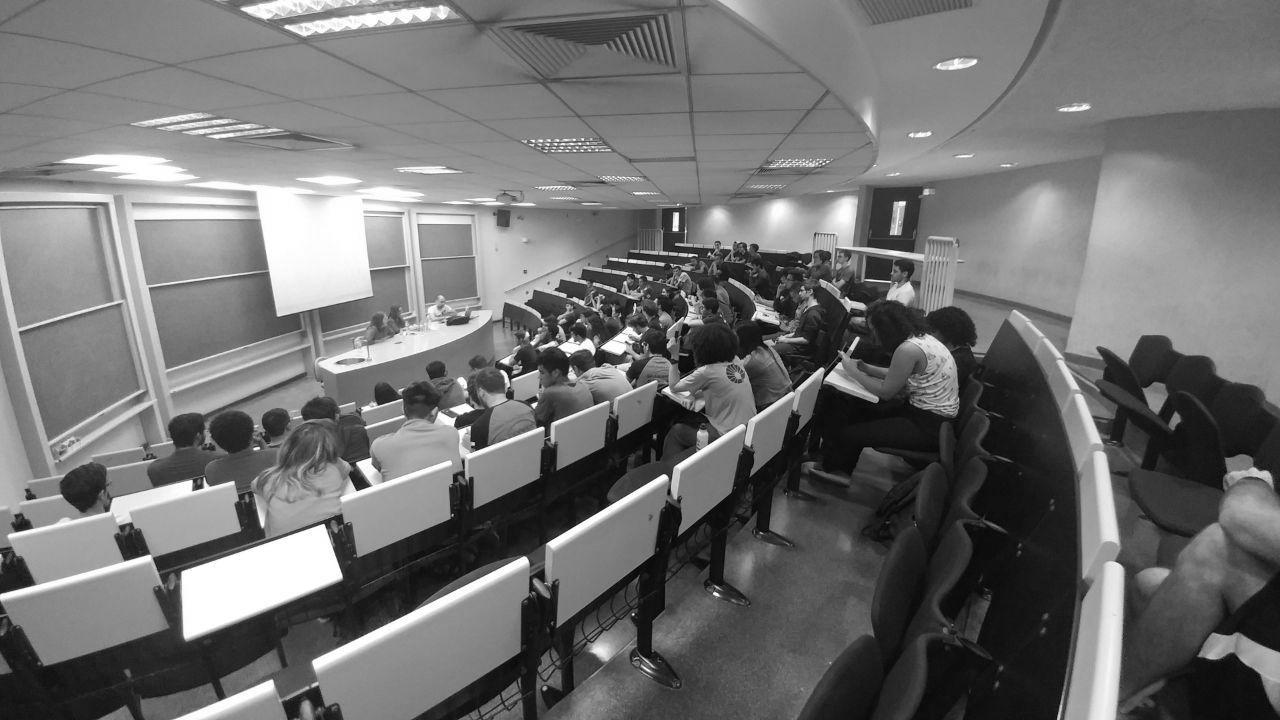
\includegraphics[width=.45\textwidth]{img/alem_da_graduacao/caco_aaab.jpg}
\end{figure}


\subsubsection{CACo Games}

O lendário torneio de jogos do CACo. Aberto a toda a computação, o CACo Games é
um ótimo evento de integração e já contou com oito edições de absoluto sucesso!
Você será informada da data do próximo.

\begin{figure}[H]
  \centering
  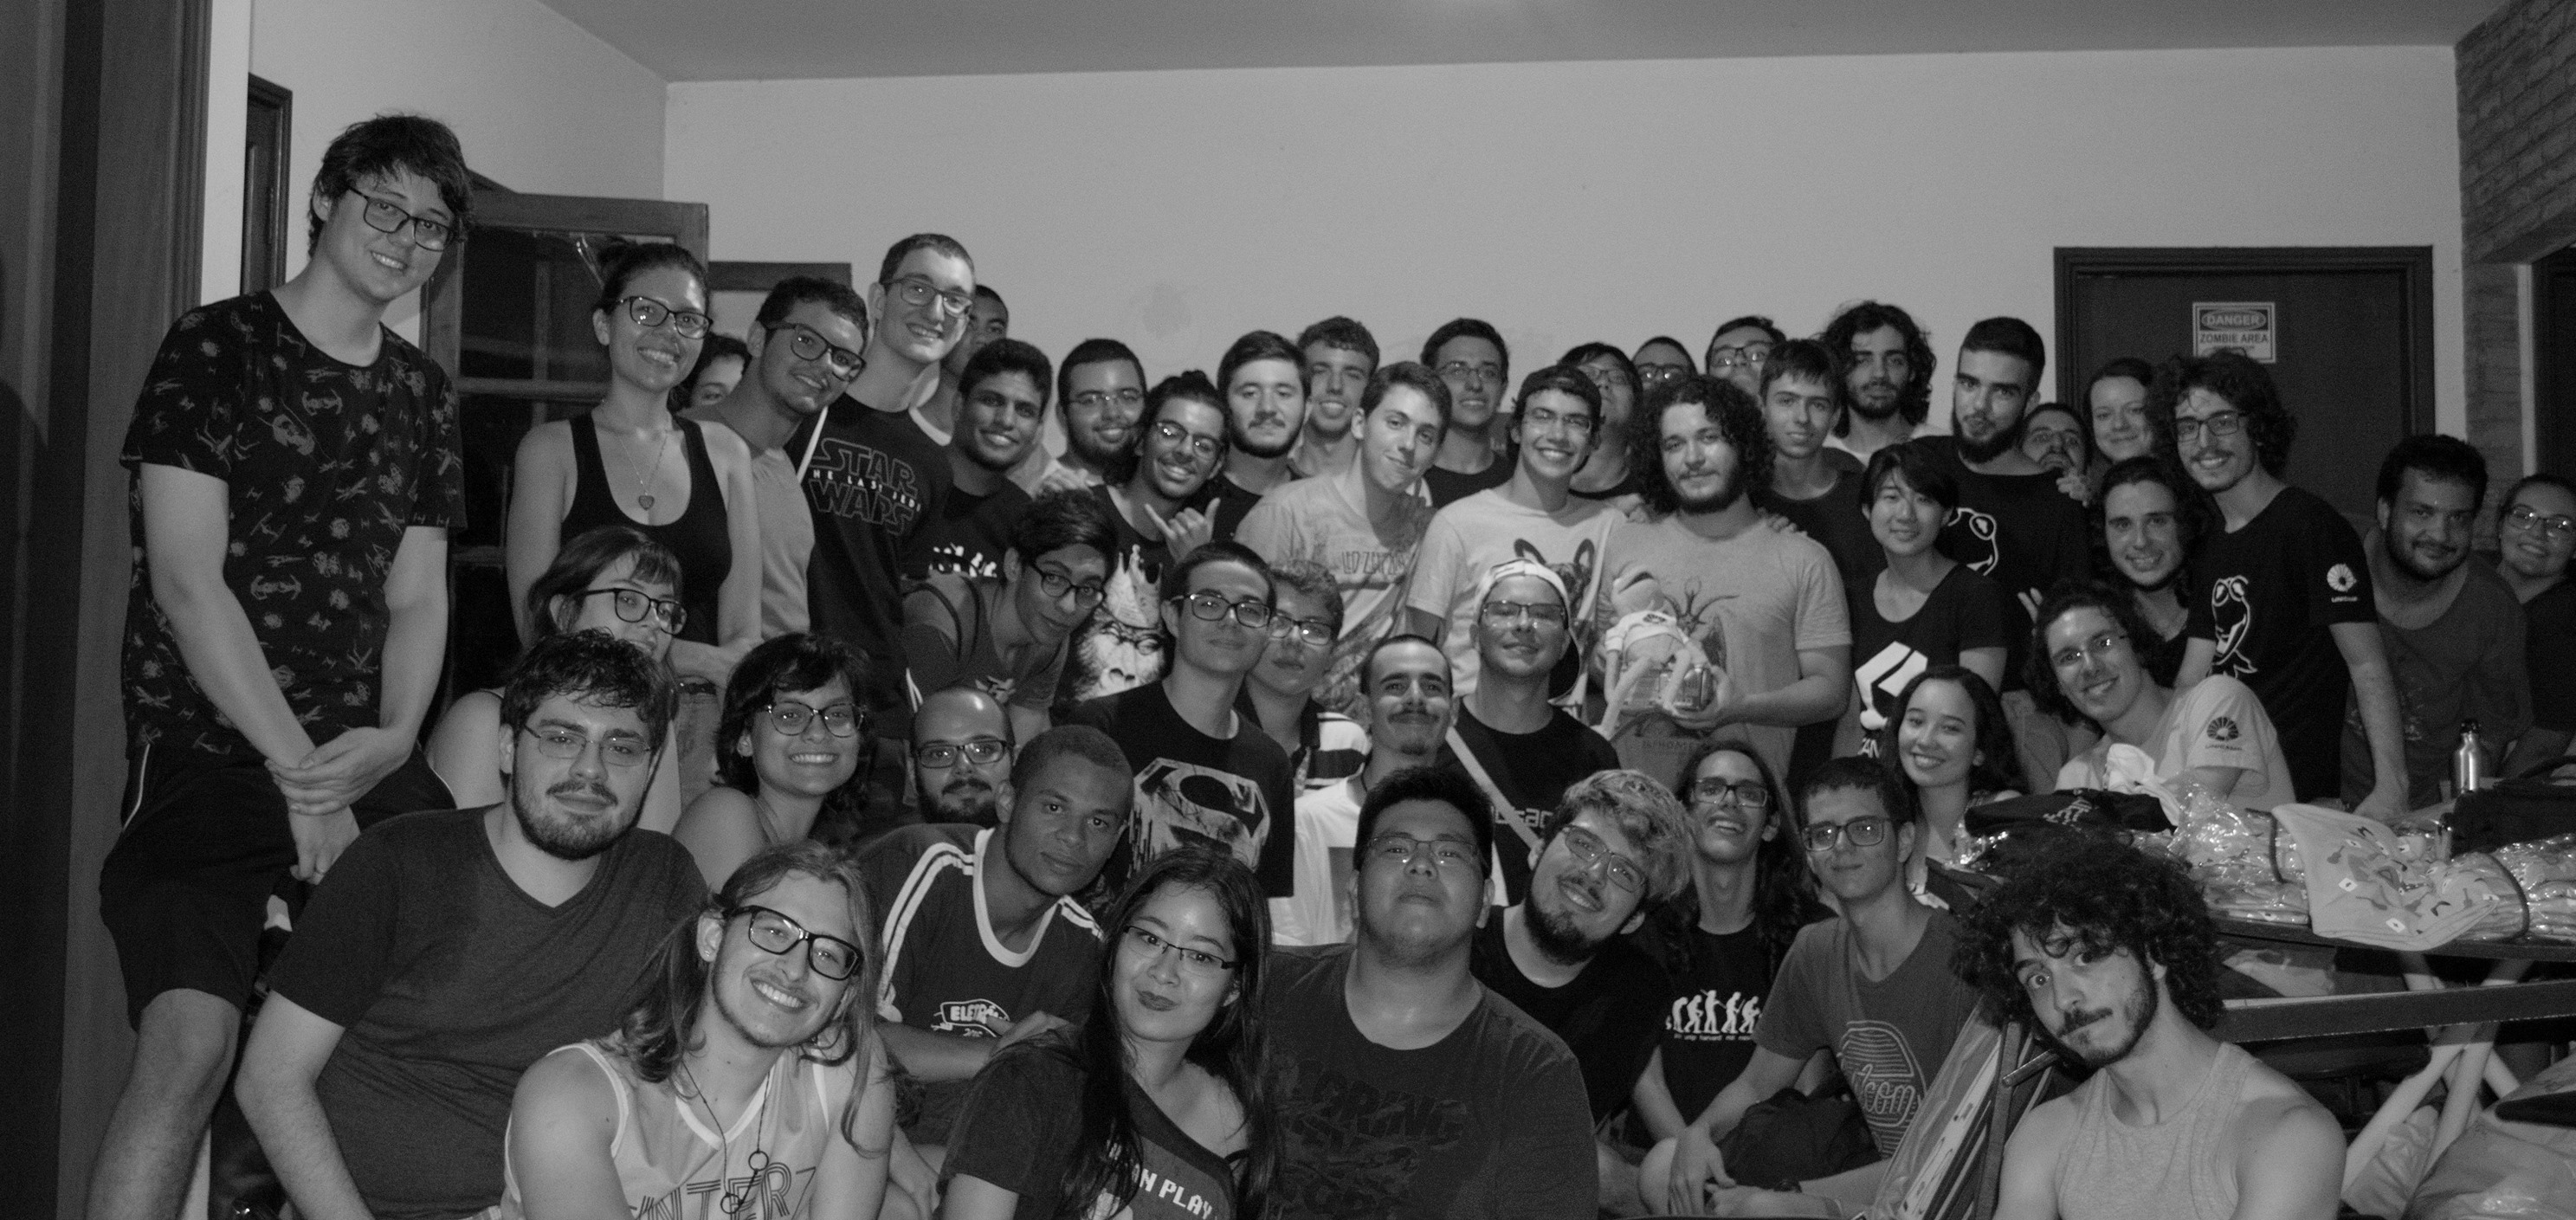
\includegraphics[width=.45\textwidth]{img/alem_da_graduacao/caco_games.jpg}
\end{figure}

\subsubsection{Manual do Bixo}

Esse excelente manual que você está lendo agora não caiu do céu. Em tempos
imemoriais, o Manual d* Bix* era feito pela Atlética, porém atualmente o CACo
assumiu a responsabilidade de editar, imprimir e distribuir o manual às
calouras e calouros todos os anos. Utilizamos Git pra controle de versão e
{\LaTeX} para formatação do conteúdo. Para contribuir, o melhor jeito é mandar
pull requests para nosso repositório,
\begin{center}
\url{github.com/cacounicamp/Manual-do-Bixo},\\
\end{center}
mas você também pode mandar um e-mail pra gen\-te com as contribuições caso
você não saiba usar Git ou \LaTeX.
